\documentclass[a4paper,11pt]{article}
\usepackage[utf8]{inputenc}
\usepackage[paper=a4paper, hmargin=1.5cm, bottom=1.5cm, top=3.5cm]{geometry}
\usepackage[T1]{fontenc}
\usepackage[spanish]{babel}
\usepackage[colorlinks=true, linkcolor=blue]{hyperref} %Links para el indice.
\usepackage{amsfonts}
\usepackage{verbatim}
\usepackage{listings}
\usepackage{caption}
\usepackage{subcaption}
\usepackage[table]{xcolor}
\usepackage{array,ragged2e}
\usepackage{color, colortbl}
\definecolor{Gray}{gray}{0.9}	 		
\usepackage[section]{placeins}
\usepackage{float}
%\usepackage{adjustbox}
\usepackage{amsmath}
\usepackage{blindtext}
\usepackage{sidecap}
\usepackage{color}
\usepackage{funcs}
\usepackage{graphicx}

% \newcommand{\real}{\hbox{\bf R}}

\title{Trabajo Práctico de Ingeniería de Software I}

\begin{document}

\maketitle

\begin{center}
	Universidad de Buenos Aires - Departamento de Computaci\'on - FCEN
\end{center}

\vspace{2cm}
Integrantes:

\begin{itemize}
	\item Castro, Dami\'an L.U.: 326/11  \verb+ltdicai@gmail.com+
	\item Matayoshi, Leandro L.U.: 79/11 \verb+leandro.matayoshi@gmail.com+
	\item Melnik, Jonathan L.U.: 571/09 \verb+jonathanmelnik@gmail.com+
	\item Santos, Martín L.U.: 413/11 \verb+martin.n.santos@gmail.com+
	\item Szyrej, Alexander L.U.: 642/11   \verb+alexanderszyrej@gmail.com+
	
\end{itemize}

\newpage

\tableofcontents

\newpage

\section{Descripción de casos de uso}

\subsection{Usuario}

~

\cu{Iniciando trámite de registración}{Usuario}{}

\begin{center}
    \centering
    \begin{tabular}{ | p{11cm} | p{6cm} | }
    	\multicolumn{1}{c}{\cellcolor{black!30}\textbf{Curso normal}} & 
    	\multicolumn{1}{c}{\cellcolor{black!30}\textbf{Curso alternativo}} \\
		\hline
		1- El sistema despliega una interfaz gráfica con campos a completar
		por el usuario: Nombre completo, Número de DNI, Domicilio, Mail y un teléfono
		para contacto en caso de ser necesario &  \\ \hline
		2 - El usuario ingresa los datos en el sistema & 2.1 - El usuario ya se encuentra ingresado en el sistema
		o hay una inconsistencia con los datos de otro usuario almacenado en la base de datos. Fin de C.U \\ \hline
		3 - El sistema registra al usuario en el sistema, almacena los datos en la base de datos y le anuncia al usuario que la registración se completará cuando los datos se validen y que se le comunicará de dicha operación via email.& \\ \hline
		\underline{Postcondición :} Trámite de registración iniciado & \\ \hline
    \end{tabular}
\end{center}

Una vez que el registro es realizado, los datos quedan sujetos a verificación por parte de un empleado de gobierno.

~

\cu{Logueándose}{Usuario}{}
\begin{center}
    \centering
    \begin{tabular}{ | p{11cm} | p{6cm} | }
    	\multicolumn{1}{c}{\cellcolor{black!30}\textbf{Curso normal}} & 
    	\multicolumn{1}{c}{\cellcolor{black!30}\textbf{Curso alternativo}} \\
		\hline
		1- El sistema despliega una interfaz gráfica con campos a completar
		por el usuario: Nombre completo, Número de DNI, Domicilio, Mail y un teléfono
		para contacto en caso de ser necesario &  \\ \hline
		2 - El usuario ingresa los datos en el sistema & 2.1 - El usuario ya se encuentra ingresado en el sistema
		o hay una inconsistencia con los datos de otro usuario almacenado en la base de datos. Fin de C.U \\ \hline
		3 - El sistema registra al usuario en el sistema y almacena los datos en la base de datos & \\ \hline
		\underline{Postcondición :} Usuario registrado & \\ \hline
    \end{tabular}
\end{center}

~

\cu{Consultando stock/tiempo}{Usuario}{Trámite de registración iniciado}
\begin{center}
    \centering
    \begin{tabular}{ | p{11cm} | p{6cm} | }
    	\multicolumn{1}{c}{\cellcolor{black!30}\textbf{Curso normal}} & 
    	\multicolumn{1}{c}{\cellcolor{black!30}\textbf{Curso alternativo}} \\
		\hline
		1- El usuario le informa al sistema que desea realizar una consulta acerca de la disponibilidad
		de bicicletas en una determinada estación & \\ \hline
		2- El sistema despliega una lista con las estaciones que es posible consultar & 
		2.1- El usuario no encuentra en la lista la estación que está buscando porque la misma no se encuentra en
		funcionamiento, con lo cual o bien procede a consultar disponibilidad en una estación cercana (ir al paso 3), o
		decide finalizar la consulta (Fin de C.U)\\ \hline
		3- El usuario selecciona la estación sobre la cual desea consultar. & \\ \hline
		4- El sistema envía información acerca de la disponibilidad en la estación seleccionada al momento de la consulta, utilizando distintos colores para reforzar el contenido del mensaje. En el caso de haber muchas bicicletas disponibles utiliza el color verde. Si hay una cantidad moderada de bicicletas utiliza el color naranja. Finalmente,
		si la cantidad de bicicletas disponibles está por agotarse utiliza el color rojo. Si por el contrario no hay
		bicicletas disponibles en la estación el sistema informa este hecho al usuario y envía un tiempo estimado en el cual
		es probable que el stock vuelva a ser positivo. & \\ \hline
		\underline{Postcondición :} Consulta realizada & \\ \hline
    \end{tabular}
\end{center}	

~

\cu{Consultando propio estado}{Usuario}{Usuario logueado}
\begin{center}
    \centering
    \begin{tabular}{ | p{11cm} | p{6cm} | }
    	\multicolumn{1}{c}{\cellcolor{black!30}\textbf{Curso normal}} & 
    	\multicolumn{1}{c}{\cellcolor{black!30}\textbf{Curso alternativo}} \\
		\hline
		1- El usuario le informa al sistema que desea consultar su estado & \\ \hline
		2- El sistema le despliega una interfaz con varias opciones a consultar:
		Si el usuario está penalizado actualmente, el historial de 
		penalizaciones y el historial de alquileres. & \\ \hline
		3- El usuario indica la opción que desea consultar & \\ \hline
		4- El sistema le envía al usuario la información solicitada.
		\underline{Postcondición :} Consulta individual realizada & \\ \hline
    \end{tabular}
\end{center}

~

\cu{Agregando sugerencia}{Usuario}{Usuario logueado}
\begin{center}
    \centering
    \begin{tabular}{ | p{11cm} | p{6cm} | }
    	\multicolumn{1}{c}{\cellcolor{black!30}\textbf{Curso normal}} & 
    	\multicolumn{1}{c}{\cellcolor{black!30}\textbf{Curso alternativo}} \\
		\hline
		1- El usuario le informa al sistema que desea enviar una sugerencia & \\ \hline
		2- El sistema despliega un cuadro de texto en donde el usuario puede escribir los comentarios,
		mostrando también las pautas del correcto uso de dicha herramienta (Solicita
		utilizar el espacio con
		responsabilidad evitando el uso indebido del lenguaje).
		También muestra ejemplos de comentarios que han ayudado a la mejora de las ciclovías. & \\ \hline
		3- El usuario ingresa sus comentarios y los envía al sistema & \\ \hline
		4- El sistema le indica al usuario que las sugerencias han sido almacenadas & \\ \hline
		\underline{Postcondición :} Sugerencia enviada & \\ \hline
    \end{tabular}
\end{center}





\cu{Validando autenticación}{Empleado de estación}{}
\begin{center}
    \centering
    \begin{tabular}{ | p{11cm} | p{6cm} | }
    	\multicolumn{1}{c}{\cellcolor{black!30}\textbf{Curso normal}} & 
    	\multicolumn{1}{c}{\cellcolor{black!30}\textbf{Curso alternativo}} \\
		\hline
		1- El empleado de estación indica al sistema que desea ver los datos del usuario. &  \\ \hline
		2- El sistema despliega una interfaz gráfica con un campo DNI a completar correspondiente al usuario. &  \\ \hline
		3- El empleado de estación ingresa el DNI del usuario. &  
		3.1- El sistema indica que el usuario no existe y permite volver al paso anterior para ingresar el DNI. Volver al paso 3. \\ \hline
		4- El sistema indica que el usuario es válido. & \\ \hline
		\underline{Postcondición :} Autenticación de usuario validada & \\ \hline
    \end{tabular}
\end{center}

~

\cu{Consultando datos de usuario}{Empleado de estación}{Autenticación de usuario validada}
\begin{center}
    \centering
    \begin{tabular}{ | p{11cm} | p{6cm} | }
    	\multicolumn{1}{c}{\cellcolor{black!30}\textbf{Curso normal}} & 
    	\multicolumn{1}{c}{\cellcolor{black!30}\textbf{Curso alternativo}} \\
		\hline
		1- El empleado de estación indica al sistema que desea ver los datos del usuario. &  \\ \hline
		2- El sistema despliega una interfaz gráfica con un campo DNI a completar correspondiente al usuario. &  \\ \hline
		3- El empleado de estación ingresa el DNI del usuario. &  \\ \hline
		4- El sistema muestra los datos del usuario correspondientes al DNI ingresado: Nombre, e-mail, teléfono y dirección. También muestra el estado del alquiler actual o un formulario para ingresar un nuevo alquiler(en caso de que no haya ningún alquiler activo), si está penalizado actualmente y un formulario para ingresar penalizaciones. & \\ \hline		
		\underline{Postcondición :} Datos de usuario consultados & \\ \hline
    \end{tabular}
\end{center}

~

\cu{Registrando retiro de bicicleta}{Empleado de estación}{}
\begin{center}
    \centering
    \begin{tabular}{ | p{11cm} | p{6cm} | }
    	\multicolumn{1}{c}{\cellcolor{black!30}\textbf{Curso normal}} & 
    	\multicolumn{1}{c}{\cellcolor{black!30}\textbf{Curso alternativo}} \\
		\hline
		1- El empleado de estación consulta los datos del usuario. Usa Consultando datos de usuario. &  \\ \hline
		2- El empleado de estación completa el formulario de alquiler, ingresando el ID de la bicicleta. Luego envía el formulario al sistema. & \\ \hline
		3- El sistema indica que el alquiler fue registrado correctamente. & \\ \hline
		\underline{Postcondición :} Retiro de bicicleta registrado & \\ \hline
    \end{tabular}
\end{center}

~

\cu{Ingresando penalización}{Empleado de estación}{}
\begin{center}
    \centering
    \begin{tabular}{ | p{11cm} | p{6cm} | }
    	\multicolumn{1}{c}{\cellcolor{black!30}\textbf{Curso normal}} & 
    	\multicolumn{1}{c}{\cellcolor{black!30}\textbf{Curso alternativo}} \\
		\hline
		1- El empleado de estación consulta los datos del usuario. Usa Consultando datos de usuario. &  \\ \hline
		2. El empleado de estación completa el formulario de penalizaciones, ingresando el tipo de penalización y algún comentario pertinente a la penalización. Luego envía el formulario al sistema. & \\ \hline
		3- El sistema indica que la penalización fue ingresada correctamente. & \\ \hline
		\underline{Postcondición :} Usuario penalizado & \\ \hline
    \end{tabular}
\end{center}

El tiempo que el usuario dure penalizado es calculado por el sistema a partir del tipo de penalización indicado.

~

\cu{Modificando stock de estación}{Empleado de estación}{}
\begin{center}
    \centering
    \begin{tabular}{ | p{11cm} | p{6cm} | }
    	\multicolumn{1}{c}{\cellcolor{black!30}\textbf{Curso normal}} & 
    	\multicolumn{1}{c}{\cellcolor{black!30}\textbf{Curso alternativo}} \\
		\hline
		1- El empleado de estación indica al sistema que desea modificar el stock de estación. & \\ \hline
		2- El sistema despliega un formulario para ingresar por separado los listados de IDs de las bicicletas que se van a agregar o remover de la estación. & \\ \hline
		3- El empleado de estación ingresa en el formulario los IDs de las bicicletas que se agregan o remueven de la estación en los campos correspondientes y envía el formulario al sistema. & \\ \hline
		4- El sistema indica el stock fue modificado correctamente. & \\ \hline
		\underline{Postcondición :} Stock de estación modificado & \\ \hline
    \end{tabular}
\end{center}	

El empleado de estación modifica el stock cuando la empresa de transportes ingresa o retira bicicletas de su estación.

~

\cu{Ingresando bicicleta en mal estado}{Empleado de estación}{}
\begin{center}
    \centering
    \begin{tabular}{ | p{11cm} | p{6cm} | }
    	\multicolumn{1}{c}{\cellcolor{black!30}\textbf{Curso normal}} & 
    	\multicolumn{1}{c}{\cellcolor{black!30}\textbf{Curso alternativo}} \\
		\hline
		1- El empleado de estación indica al sistema que desea modificar el estado de una bicicleta. & \\ \hline
		2- El sistema muestra un formulario con los campos ID y estado, donde ID es el de la bicicleta y estado es un campo de texto para ingresar el detalle del estado de la bicicleta. & \\ \hline
		3- El empleado de estación completa el formulario y lo envía. & \\ \hline
		4- El sistema indica que se ingresó correctamente el cambio de estado de la bicicleta. & \\ \hline
		\underline{Postcondición :} Bicicleta en mal estado ingresada & \\ \hline
    \end{tabular}
\end{center}

~

\cu{Registrando devolución de bicicleta}{Empleado de estación}{}
\begin{center}
    \centering
    \begin{tabular}{ | p{11cm} | p{6cm} | }
    	\multicolumn{1}{c}{\cellcolor{black!30}\textbf{Curso normal}} & 
    	\multicolumn{1}{c}{\cellcolor{black!30}\textbf{Curso alternativo}} \\
		\hline
		1- El empleado de estación consulta los datos del usuario. Usa Consultando datos de usuario. &  \\ \hline
		2- El empleado de estación actualiza el estado del alquiler del usuario para reflejar que la bicicleta fue devuelta exitosamente.
		3- Si la bicicleta está en mal estado, el empleado de estación penaliza al usuario(extiende Ingresando Penalización) e ingresa la bicicleta en mal estado al sistema(extiende Ingresando bicicleta en mal estado).		
		4- Si el tiempo de alquiler fue excedido, el empleado de estación penaliza al usuario por demora(extiende Ingresando Penalización).
		\underline{Postcondición :} Devolución de bicicleta registrada & \\ \hline
    \end{tabular}
\end{center}


\subsection{Empleado de gobierno}

~

\cu{Ingresando nueva estación}{Empleado de gobierno}{}

\begin{center}
    \centering
    \begin{tabular}{ | p{11cm} | p{6cm} | }
    	\multicolumn{1}{c}{\cellcolor{black!30}\textbf{Curso normal}} & 
    	\multicolumn{1}{c}{\cellcolor{black!30}\textbf{Curso alternativo}} \\ \hline
    	1- El empleado de gobierno indica al sistema que desea agregar una nueva estación & \\ \hline
    	2- El sistema despliega una interfaz con campos a completar necesarios para el registro de la 
    	nueva estación: nombre, dirección y capacidad de la misma. & \\ \hline
    	3- El empleado completa los datos y los envía al sistema & 3.1- Alguno de los campos es incorrecto:
    	Ya existe una estación en el sistema con dicho nombre o dirección, o la capacidad es incorrecta:
    	menor a la mínima - superior a la máxima. Volver al paso 3. \\ \hline
    	4- El sistema le indica al empleado que la estación fue registrada correctamente
		\underline{Postcondición :} Estación agregada & \\ \hline
    \end{tabular}
\end{center}

~

\cu{Consultando estadísticas}{Empleado de gobierno}{}

\begin{center}
    \centering
    \begin{tabular}{ | p{11cm} | p{6cm} | }
    	\multicolumn{1}{c}{\cellcolor{black!30}\textbf{Curso normal}} & 
    	\multicolumn{1}{c}{\cellcolor{black!30}\textbf{Curso alternativo}} \\ \hline
    	1- El empleado de gobierno indica al sistema que desea consultar una estadística. & \\ \hline
    	2- El sistema despliega una interfaz con las posibles estadísticas a consultar. & \\ \hline
    	3- El empleado selecciona la estadística de interés, junto con un rango temporal sobre el cual
    	desea consultar. (Último día, semana, mes, año o histórico) & \\ \hline
    	4- El sistema despliega la información solicitada. & \\ \hline
		\underline{Postcondición :} Estadística consultada & \\ \hline
    \end{tabular}
\end{center}

~

\cu{Consultando sugerencias}{Empleado de gobierno}{}

\begin{center}
    \centering
    \begin{tabular}{ | p{11cm} | p{6cm} | }
    	\multicolumn{1}{c}{\cellcolor{black!30}\textbf{Curso normal}} & 
    	\multicolumn{1}{c}{\cellcolor{black!30}\textbf{Curso alternativo}} \\ \hline
    	1- El empleado de gobierno indica al sistema que desea ver sugerencias hechas por los usuarios. & \\ \hline
    	2- El sistema despliega una interfaz con varias opciones: Por un lado puede elegir consultar. 
    	las sugerencias de todos los usuarios, o seleccionar uno específico ingresando su DNI. Al mismo
    	tiempo puede filtrar las consultas por rango temporal (Realizadas el último día, semana, mes, año
    	o histórico). & \\ \hline
    	3- El empleado selecciona el modo de consulta. & 3.1- El usuario ingresa un DNI que no pertenece a ningún usuario. Volver al paso 2. \\ \hline
    	4- El sistema envía las sugerencias solicitadas. & \\ \hline
	\underline{Postcondición :} Sugerencias consultadas & \\ \hline
    \end{tabular}
\end{center}

~

\cu{Actualizando estado de la empresa de transportes}{Empleado de gobierno}{}

\begin{center}
    \centering
    \begin{tabular}{ | p{11cm} | p{6cm} | }
    	\multicolumn{1}{c}{\cellcolor{black!30}\textbf{Curso normal}} & 
    	\multicolumn{1}{c}{\cellcolor{black!30}\textbf{Curso alternativo}} \\ \hline
    	1- El empleado de gobierno indica al sistema que desea ingresar información relevante respecto a la empresa de transportes & \\ \hline
    	2- El sistema despliega una interfaz con dos posibles opciones para completar: Advertir inactividad de la empresa durante cierto rango de tiempo,
    	o actualizar la cantidad de camiones disponibles para traslados durante cierto rango de tiempo & \\ \hline
    	3- El empleado de gobierno selecciona la opción que desea e ingresa los datos. & \\ \hline
	\underline{Postcondición :} Actualización completada & \\ \hline
    \end{tabular}
\end{center}

Si el empleado de gobierno ingresara Inactividad de la empresa entre 15:00 y 17:00hs estaría indicándole al sistema que la empresa de transportes no realizará ningún
traslado de bicicletas durante dicho horario.
Si el empleado ingresara 20 camiones entre las 15:00 y 17:00hs estaría indicándole al sistema que la empresa de transportes destinará 20 de sus camiones para traslados
de bicicletas durante dicho horario.

~

\cu{Ingresando nuevas bicicletas}{Empleado de gobierno}{}

\begin{center}
    \centering
    \begin{tabular}{ | p{11cm} | p{6cm} | }
    	\multicolumn{1}{c}{\cellcolor{black!30}\textbf{Curso normal}} & 
    	\multicolumn{1}{c}{\cellcolor{black!30}\textbf{Curso alternativo}} \\ \hline
    	1- El empleado de gobierno indica al sistema que desea registrar el ingreso de nuevas bicicletas & \\ \hline
    	2- El sistema despliega una interfaz en donde permite seleccionar la cantidad de bicicletas, el tipo de las mismas y el rango Id correspondiente.& \\ \hline
    	3- El empleado de gobierno ingresa los datos & 3.1-  Alguno de los campos es incorrecto. Por ejemplo:
        ya existe una bicicleta en el sistema con el mismo ID. Volver al paso 3. \\ \hline
    	4- El sistema informa que los datos han sido correctamente actualizados & \\ \hline
    	\underline{Postcondición :} Nuevas bicicletas ingresadas & \\ \hline
    \end{tabular}
\end{center}

~

\cu{Validando registro}{Empleado de gobierno}{}

\begin{center}
    \centering
    \begin{tabular}{ | p{11cm} | p{6cm} | }
    	\multicolumn{1}{c}{\cellcolor{black!30}\textbf{Curso normal}} & 
    	\multicolumn{1}{c}{\cellcolor{black!30}\textbf{Curso alternativo}} \\ \hline
    	1- El empleado de gobierno indica al sistema que desea obtener el listado de las personas registradas no verificadas & \\ \hline
    	2- El sistema envía el listado & \\ \hline
    	3- El empleado selecciona alguna de las entradas para validarla & \\ \hline
    	4- El sistema despliega la información presentada por el usuario al momento del registro & \\ \hline
    	5- El empleado indica que la información es válida & 5.1- El empleado encuentra una anomalía en los datos e indica qué información es inválida. El sistema notifica por mail al usuario
    	informándole los datos de registro inválidos y le solicita que se registre nuevamente \\ \hline
    	6- El sistema informa al empleado de gobierno que la validación se completó exitosamente & \\ \hline
    	\underline{Postcondición :} Registación de usuario completa & \\ \hline
    \end{tabular}
\end{center}

Luego de que un usuario se registra los datos quedan sujetos a verificación por parte de un empleado de gobierno. El mismo chequea consistencia entre la documentación presentada.
En caso de encontrar alguna anomalía invalida al registro y el sistema envía una notificación al usuario. En el caso de que la validación sea exitosa, el sistema le envía un mail
al usuario informándole que la validación ha sido completada con éxito.
~






\section{Invariantes en OCL}

\oclInv{Bicicleta}{Pedido.allInstances() $\rightarrow$ forAll(p1 | Pedido.allInstances() $\rightarrow$ forAll(p2 | p1.bicicletas $\rightarrow$ includes(self) $\wedge$ p2.bicicletas $\rightarrow$ includes(self) implies p1.horaSalida $\neq$ p2.horaSalida))}{No hay una bicicleta que esté en dos pedidos distintos para una misma hora}

~

\oclInv{Bicicleta}{(Bicicleta.allInstances() $\rightarrow$ select(b | b.id = self.id) $\rightarrow$ size() ) = 1}{Los identificadores de las bicicletas son distintos}

~

\oclInv{Usuario}{(Usuario.allInstances() $\rightarrow$ select(u | u.DNI = self.DNI) $\rightarrow$ size() ) = 1}{Los DNI's de los usuarios son distintos}

~

\oclInv{Usuario}{(self.penalizacion() $\rightarrow$ size() = 1) implies (
(self.alquiler $\rightarrow$ size() = 1) implies ((self.alquiler.fecha \ < \ self.penalizacion().fechaEmision $\lor$
self.alquiler.fecha \ > \ self.penalizacion.fechaVencimiento))))}{Si un usuario está penalizado, no puede alquilar bicicletas entre
la fecha de origen de la penalización y la fecha de vencimiento}

~

\oclInv{Estacion}{(Estacion.allInstances() $\rightarrow$ select (e| e.nombre = self.nombre) $\rightarrow$ size() ) = 1}
{No hay estaciones con nombres iguales}

~

\oclInv{Estacion}{(Estacion.allInstances $\rightarrow$ select(e | e.direccion = self.direccion) -> size() ) = 1}
{No hay estaciones con direcciones iguales}
	
~

\oclInv{Pedido}{self.estacionOrigen $\neq$ self.estacionDestino}{No hay pedidos con una misma estación como origen y destino}

~

\oclInv{Pedido}{(self.bicicletas $\rightarrow$ size()) < self.estacionOrigen.capacidad}{La estación origen tiene suficiente
capacidad como para albergar la cantidad de bicicletas a retirar requerida}

~

\oclInv{Pedido}{(self.bicicletas $\rightarrow$ size()) < self.estacionDestino.capacidad}{La estación destino tiene suficiente
capacidad para albergar la cantidad de bicicletas pedidas}

~

\oclInv{Pedido}{( (self.bicicletas $\rightarrow$ forAll(b | ((b.alquiler $\rightarrow$ size() = 1) implies
(b.alquiler.Hora $\neq$ self.HoraSalida))))) }{Solo se pueden transportar bicicletas que no estén alquiladas}

~

\oclInv{EmpleadoEstacion}{(Estacion.allInstances() $\rightarrow$ select ( e | e $\rightarrow$ (includes(self))) 
$\rightarrow$ size()) = 1 }{No puede haber empleados de estación iguales que trabajen en estaciones distintas}

~

\oclInv{EstacionCentro}{(EstacionPerifera.allInstances()) $\rightarrow$ forAll(e | e.capacidad*2 $\leq$ self.capacidad)}{
Las estaciones del centro tienen más capacidad que las de la periferia. (La proporción del doble parece una aproximación
razonable)}










\section{Fsm}

\subsection{Aclaraciones de sintaxis}

Para mayor claridad y simpleza de las FSM, decidimos utilizar un abuso de notaci\'on para evitar escribir multiples transiciones.

\begin{figure}[H]
	\centering
	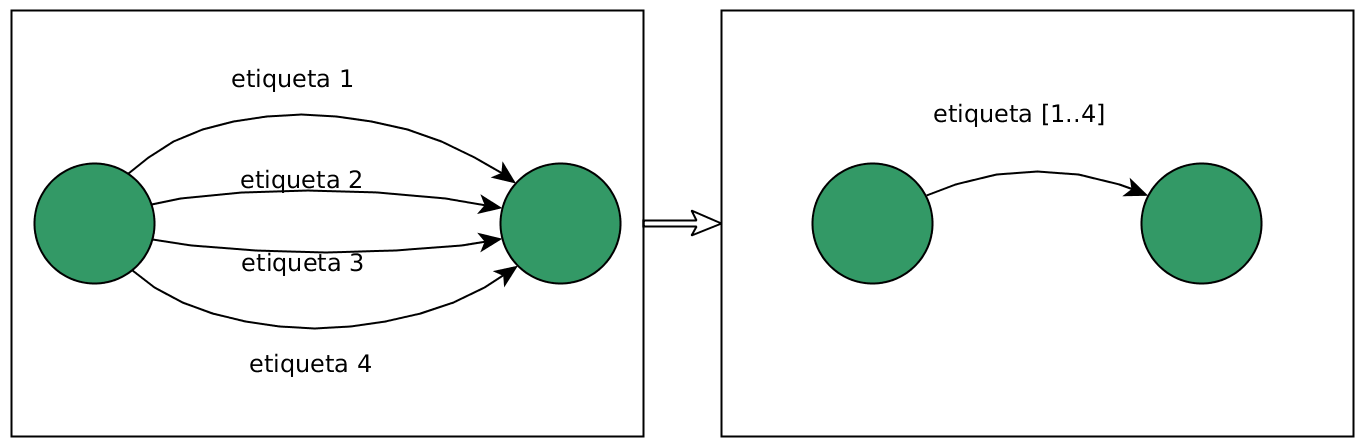
\includegraphics[scale=0.35]{imgs/fsm_ej1.png}
	\caption{Las transiciones numeradas con mismo nombre fueron reemplazadas por una \'unica transici\'on.}
\end{figure}

\begin{figure}[H]
	\centering
	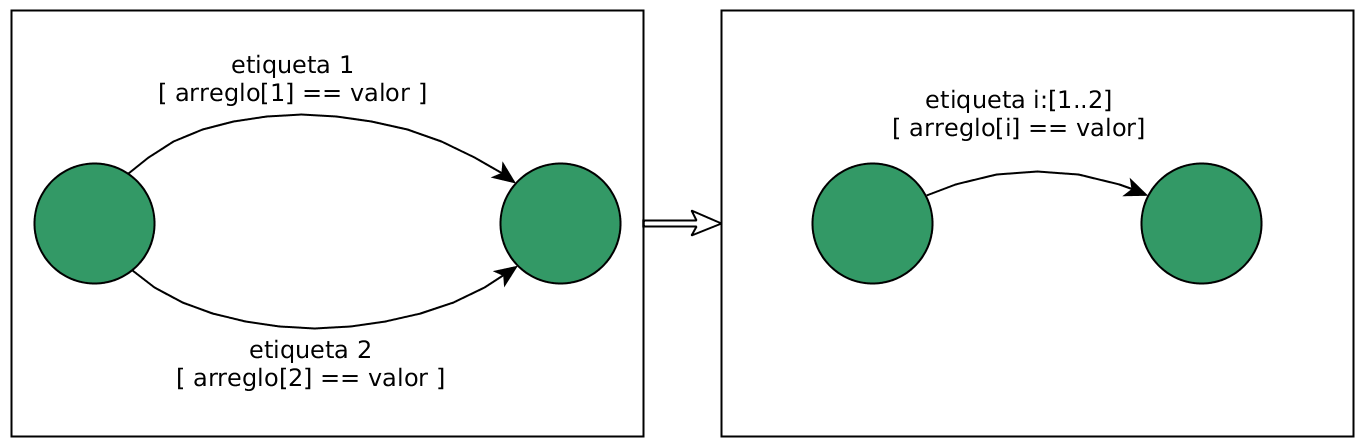
\includegraphics[scale=0.35]{imgs/fsm_ej2.png}
	\caption{Si en alg\'un momento deb\'iamos predicar sobre los n\'umeros en las etiquetas, le agregamos un iterador a la secuencia.}
\end{figure}

\subsection{Constantes y variables}

Constantes:
\begin{itemize}
\item CANT\_STOCK\_MAX es la cantidad máxima de stock en una estación. 
\item N es la cantidad de estaciones
\item M es la cantidad de habitantes en la ciudad
\item P es la cantidad total de empleados
\item ESTACION es un arreglo de P posiciones, donde ESTACION[e] es el número de la estación donde trabaja el empleado e.
\end{itemize}

Variables:
\begin{itemize}
\item stock[1..N]: [0..CANT\_STOCK\_MAX]
dasdasd
\item dondeEsta[1..M]: [0..N]. Indica, para cada usuario, en que estaci\'on se encuentra (si no se encuentra en ninguna estaci\'on el valor es 0).
\item pedido[1..N]: [-CANT\_STOCK\_MAX..CANT\_STOCK\_MAX]. Indica la cantidad de bicicletas que son enviadas a una estaci\'on. Si es para hacer un retiro de bicicletas el n\'umero es negativo. Una vez que el pedido llega o se va de la estaci\'on, el valor pasa a ser 0.
\item llegoPedido[1..N]: [0..1]. Cuando se recibe un pedido en una estaci\'on se pone el valor en 1, sino es 0.
\item atendidoPor[1..M]: [0..P]. Indica, para cada usuario, cu\'al es el empleado que lo est\'a atendiendo. Si a\'un no fue atendido, el valor es 0.
\end{itemize}

\subsection{FSM Sistema}

\begin{figure}[H]
	\centering
	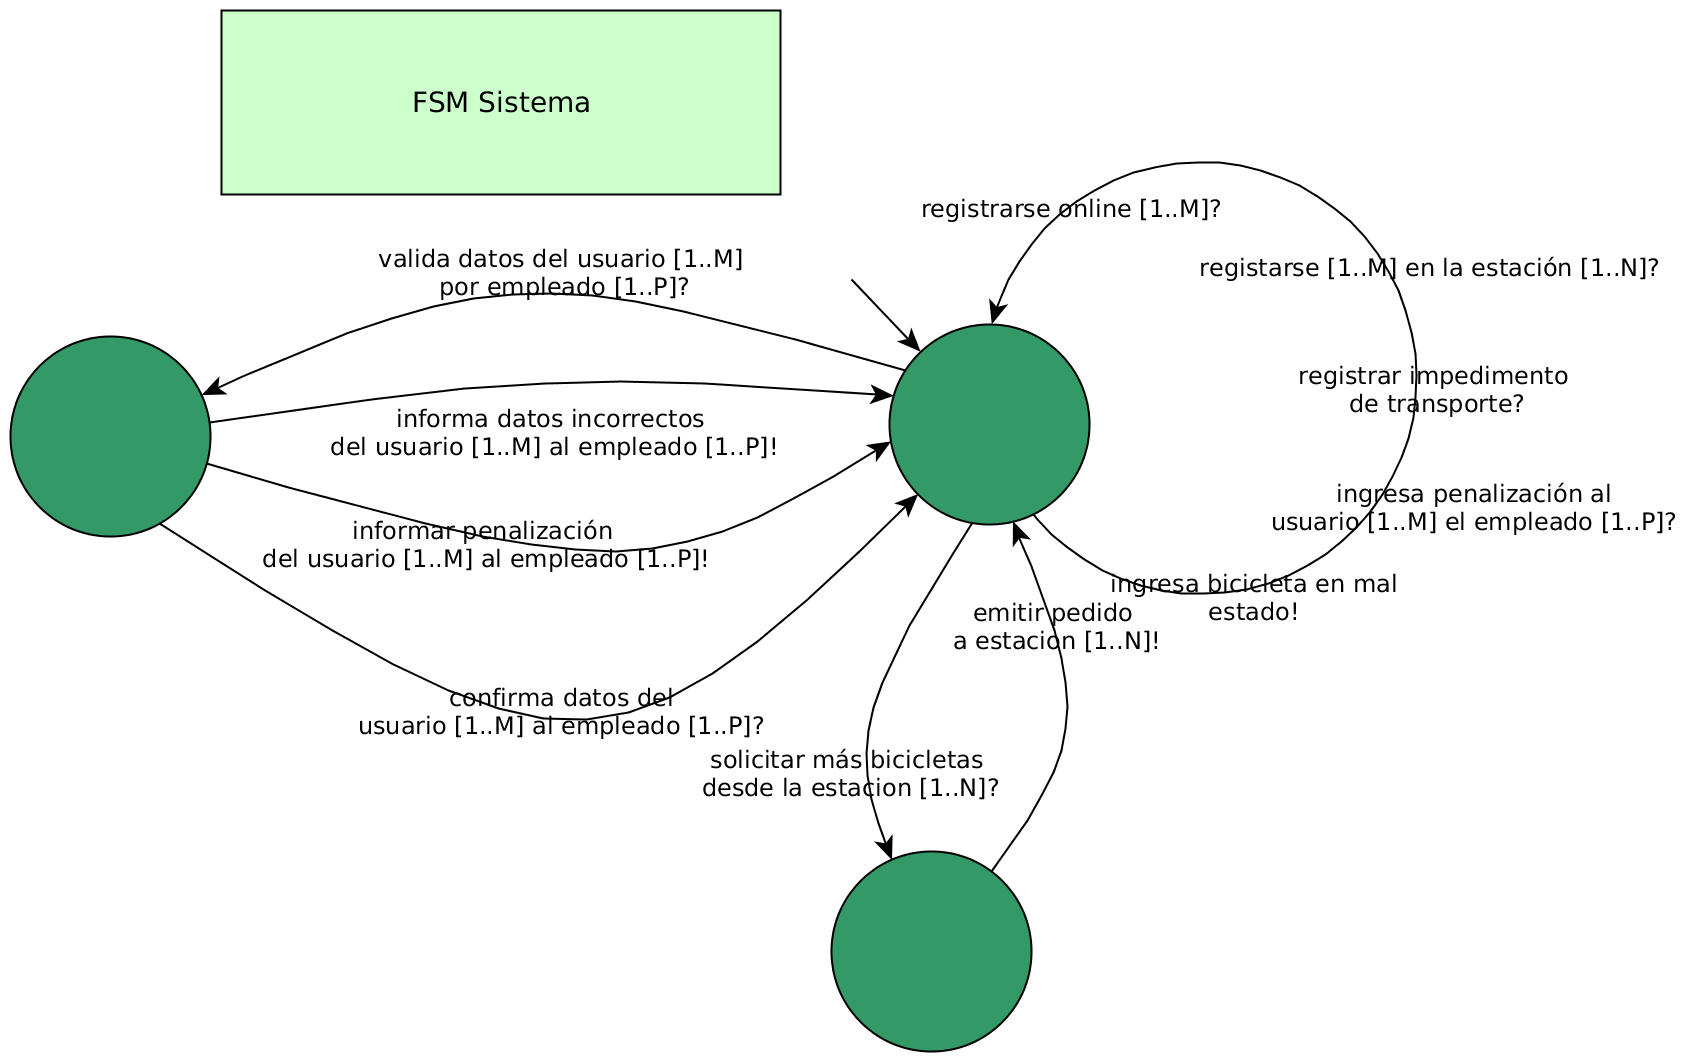
\includegraphics[scale=0.3]{imgs/fsm_sistema.png}
	\caption{FSM Sistema}
\end{figure}

\subsection{FSM Empresa de transporte}

\begin{figure}[H]
	\centering
	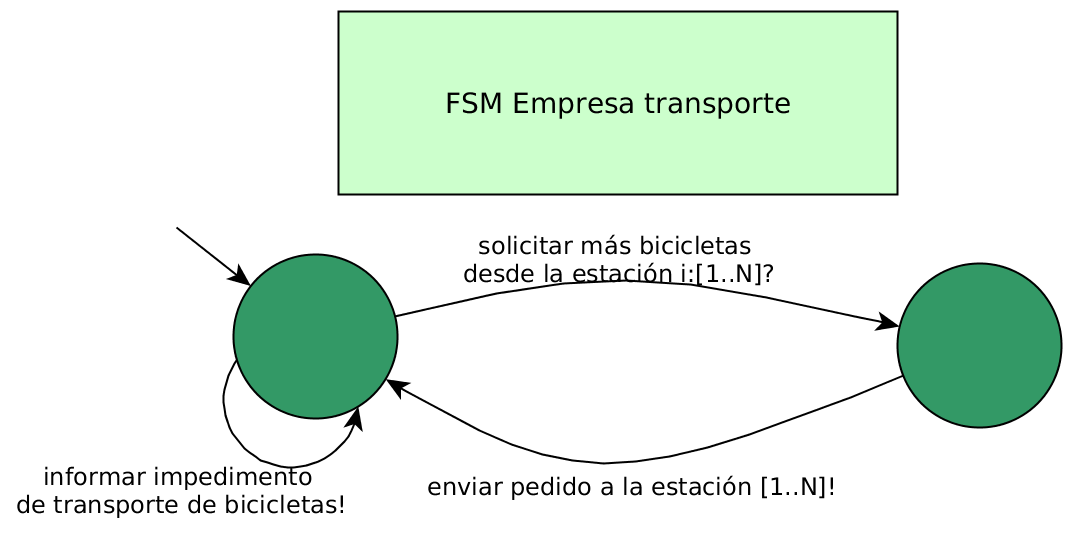
\includegraphics[scale=0.4]{imgs/fsm_empresa_transporte.png}
	\caption{FSM Empresa de transporte}
\end{figure}

\subsection{FSM Estaci\'on}

\begin{figure}[H]
	\centering
	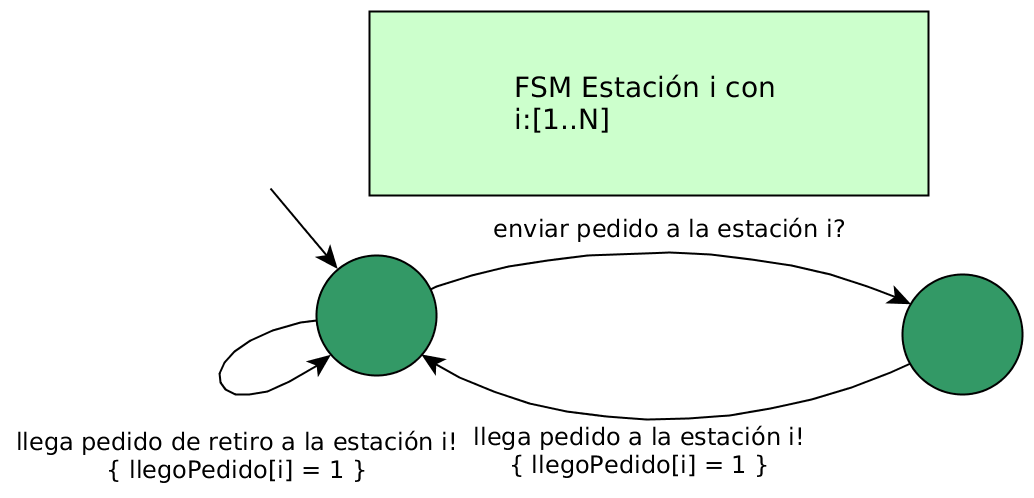
\includegraphics[scale=0.5]{imgs/fsm_estacion.png}
	\caption{FSM Estaci\'on}
\end{figure}

\subsection{FSM Controlador de stock}

\begin{figure}[H]
	\centering
	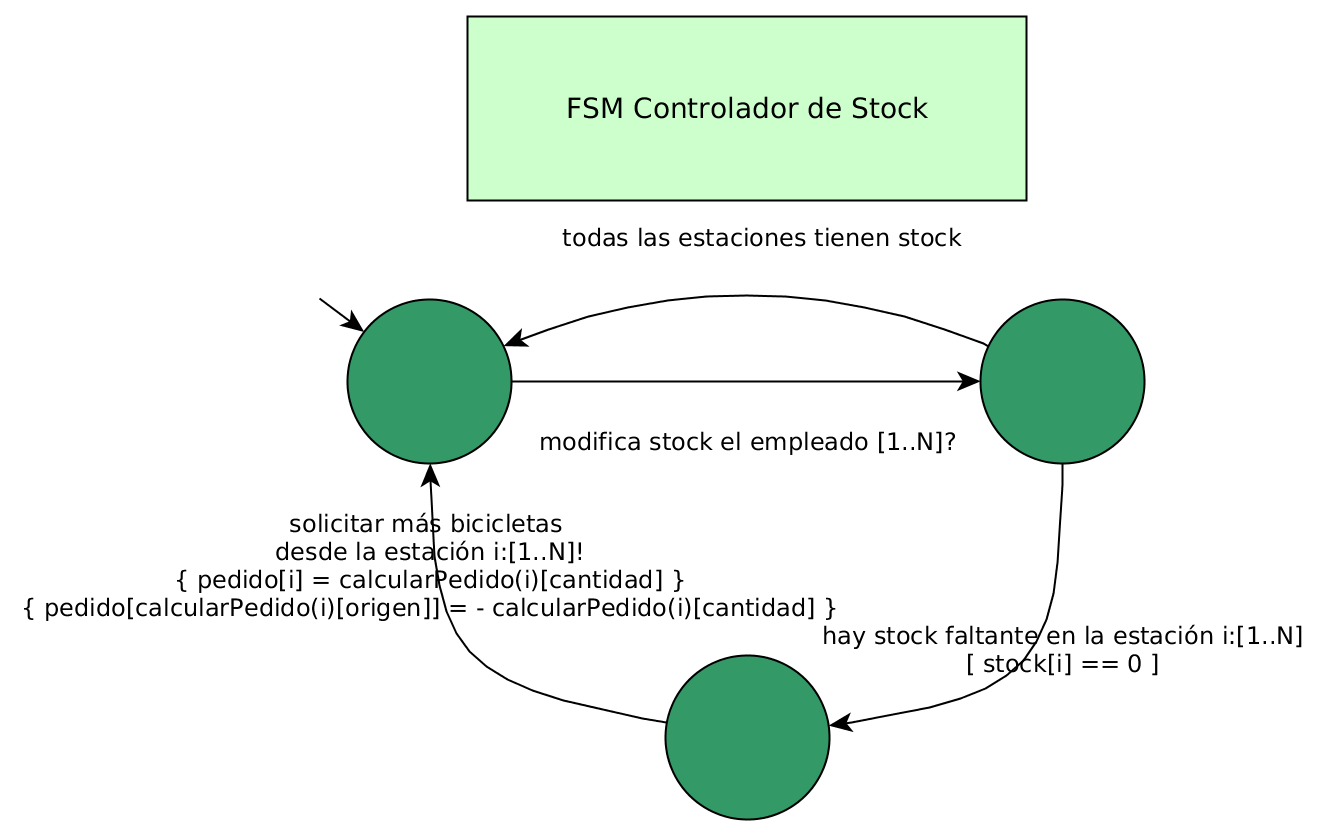
\includegraphics[scale=0.4]{imgs/fsm_controlador_stock.png}
	\caption{FSM Controlador de stock. \emph{calcularPedido(i)} es una funci\'on interna del sistema que calcula la cantidad de bicicletas a enviar\emph{([cantidad])} y desde d\'onde traerlas\emph{([origen])}.}
\end{figure}

Esta m\'aquina es una funcionalidad particular del sistema que dedicimos seperar para exhibir su comportamiento. Cada vez que un empleado modifica el stock de su estaci\'on, el controlador de stock se encarga de ver si la estaci\'on no m\'as bicicletas disponibles. En caso de ser as\'i, le avisa al sistema de que debe emitir un pedido de bicicletas. 

\subsection{FSM Empleado de gobierno}

\begin{figure}[H]
	\centering
	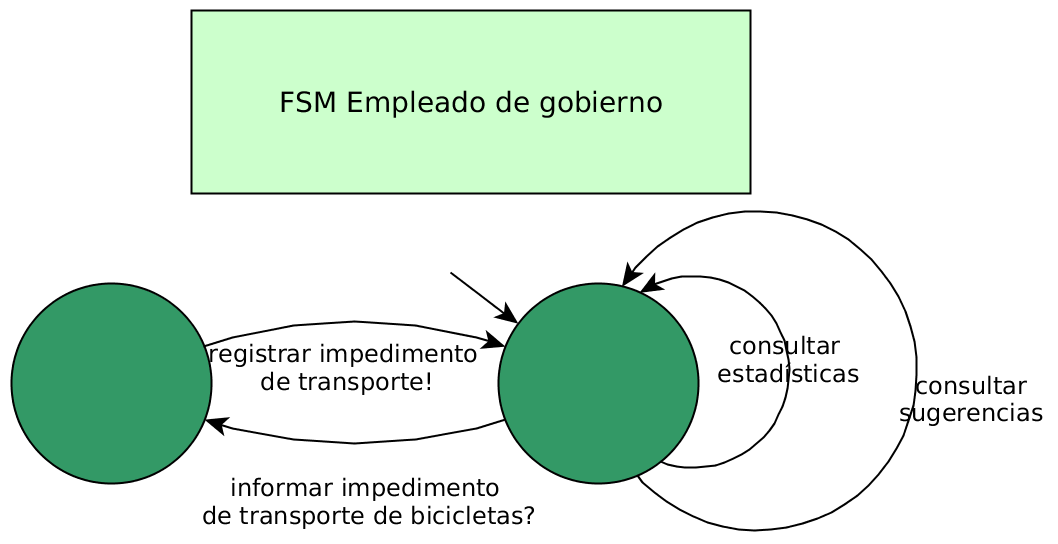
\includegraphics[scale=0.4]{imgs/fsm_empleado_gobierno.png}
	\caption{FSM Empleado de gobierno}
\end{figure}

\subsection{FSM Usuario}

\begin{figure}[H]
	\centering
	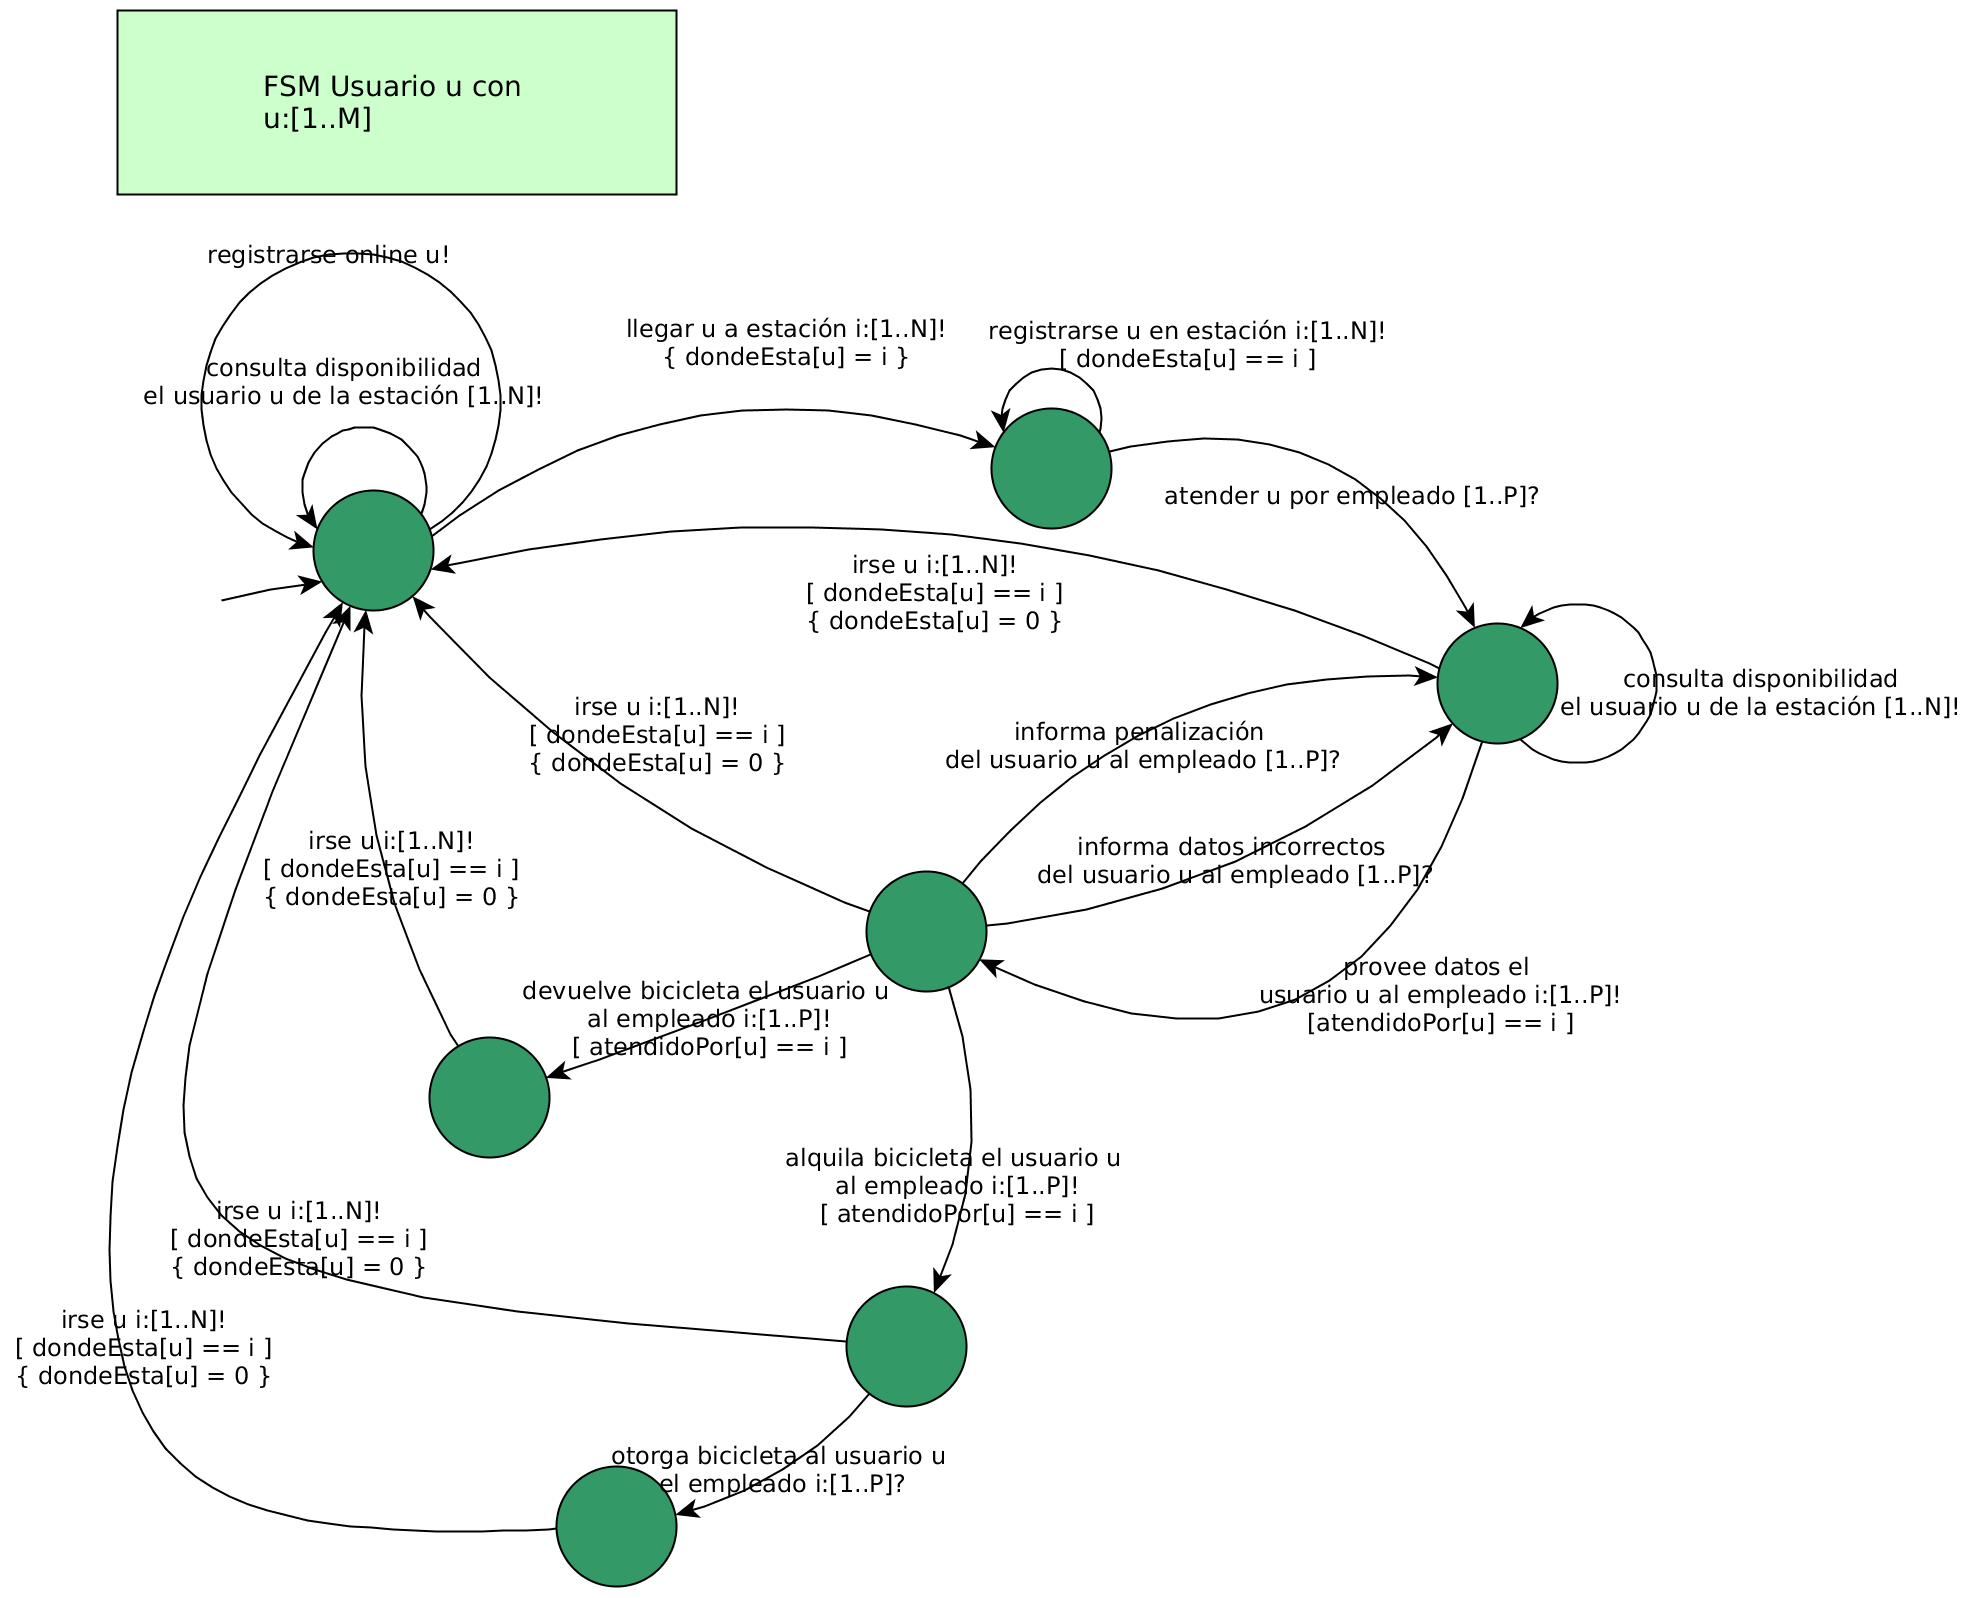
\includegraphics[scale=0.255]{imgs/fsm_usuario.png}
	\caption{FSM Usuario}
\end{figure}

\subsection{FSM Empleado}

\begin{figure}[H]
	\centering
	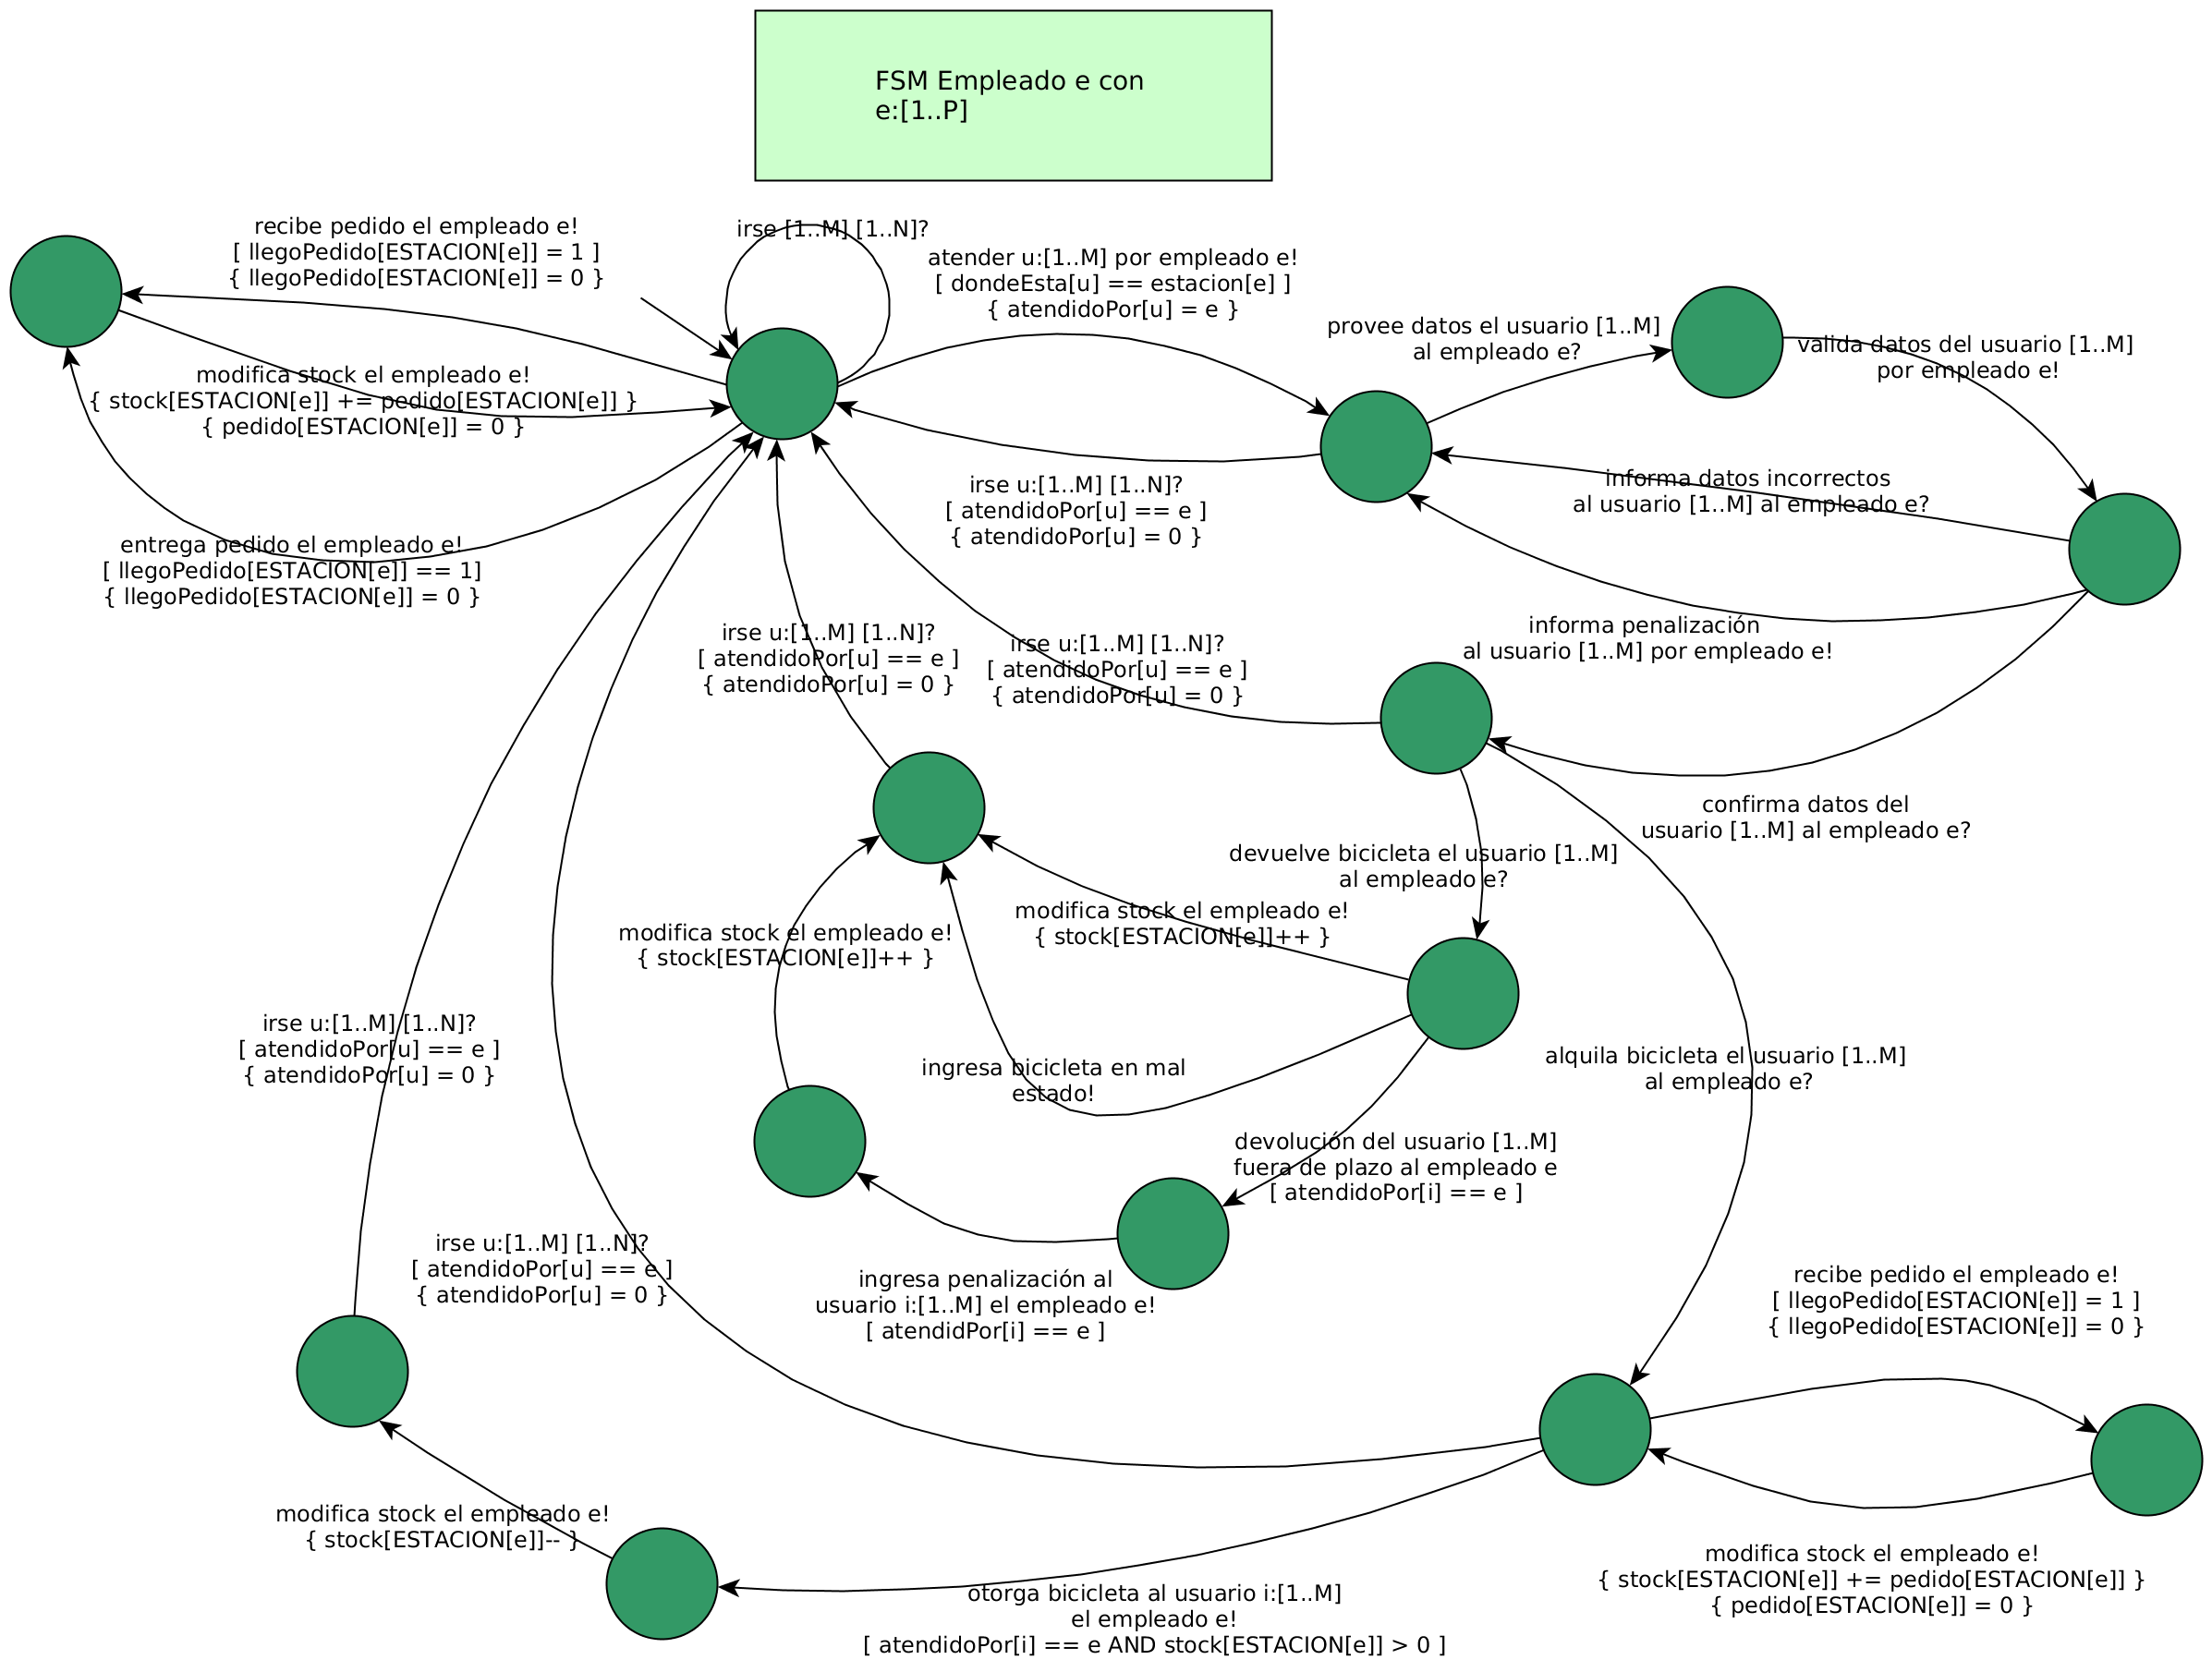
\includegraphics[scale=0.21]{imgs/fsm_empleado.png}
	\caption{FSM Empleado}
\end{figure}

\end{document}
